\section{Network Synthesis}
\paragraph{Program Synthesis: } Learning a function from specifications (e.g. examples).
In this section we cover the synthesis of correct network configurations through incorporation of powerful SAT/SMT solvers. Two such network conficuration synthesisers are SyNET and NetComplete.

\subsection{SyNET}
\begin{minipage}{\linewidth}
    \centering      
    \def\svgwidth{\linewidth}
    %% Creator: Inkscape 1.0 (4035a4fb49, 2020-05-01), www.inkscape.org
%% PDF/EPS/PS + LaTeX output extension by Johan Engelen, 2010
%% Accompanies image file 'L9_SyNET.pdf' (pdf, eps, ps)
%%
%% To include the image in your LaTeX document, write
%%   \input{<filename>.pdf_tex}
%%  instead of
%%   \includegraphics{<filename>.pdf}
%% To scale the image, write
%%   \def\svgwidth{<desired width>}
%%   \input{<filename>.pdf_tex}
%%  instead of
%%   \includegraphics[width=<desired width>]{<filename>.pdf}
%%
%% Images with a different path to the parent latex file can
%% be accessed with the `import' package (which may need to be
%% installed) using
%%   \usepackage{import}
%% in the preamble, and then including the image with
%%   \import{<path to file>}{<filename>.pdf_tex}
%% Alternatively, one can specify
%%   \graphicspath{{<path to file>/}}
%% 
%% For more information, please see info/svg-inkscape on CTAN:
%%   http://tug.ctan.org/tex-archive/info/svg-inkscape
%%
\begingroup%
  \makeatletter%
  \providecommand\color[2][]{%
    \errmessage{(Inkscape) Color is used for the text in Inkscape, but the package 'color.sty' is not loaded}%
    \renewcommand\color[2][]{}%
  }%
  \providecommand\transparent[1]{%
    \errmessage{(Inkscape) Transparency is used (non-zero) for the text in Inkscape, but the package 'transparent.sty' is not loaded}%
    \renewcommand\transparent[1]{}%
  }%
  \providecommand\rotatebox[2]{#2}%
  \newcommand*\fsize{\dimexpr\f@size pt\relax}%
  \newcommand*\lineheight[1]{\fontsize{\fsize}{#1\fsize}\selectfont}%
  \ifx\svgwidth\undefined%
    \setlength{\unitlength}{720.00000454bp}%
    \ifx\svgscale\undefined%
      \relax%
    \else%
      \setlength{\unitlength}{\unitlength * \real{\svgscale}}%
    \fi%
  \else%
    \setlength{\unitlength}{\svgwidth}%
  \fi%
  \global\let\svgwidth\undefined%
  \global\let\svgscale\undefined%
  \makeatother%
  \begin{picture}(1,0.75)%
    \lineheight{1}%
    \setlength\tabcolsep{0pt}%
    \put(0,0){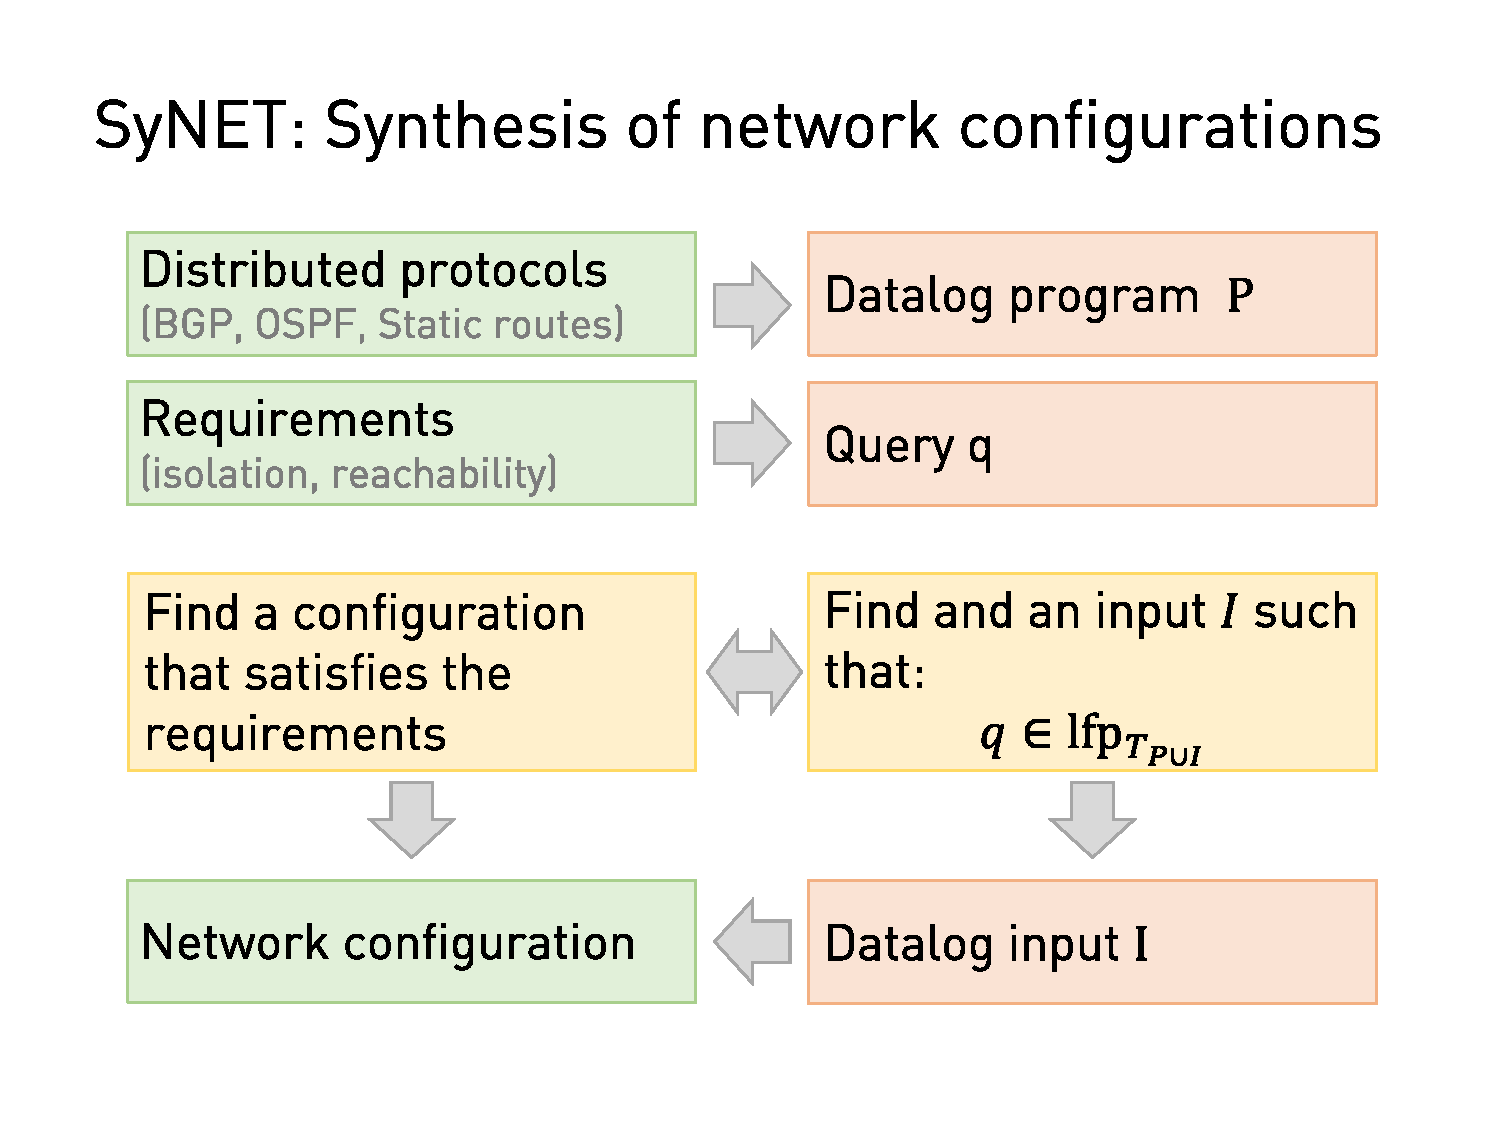
\includegraphics[width=\unitlength,page=1]{L9_SyNET.pdf}}%
  \end{picture}%
\endgroup%
    
\end{minipage}

\paragraph{Datalog rules vs SMT constraints: } Datalog rules are logical constraints that can be fed to an SMT solver.
\begin{itemize}
    \item constraints on datalog inputs (i.e. containing no derived datalog rules) can be converted directly to logical constraints.
    \item Derived datalog rules need a bit more work (unrolling) because the datalog derivation works different than the logical implication. 
\end{itemize}

\paragraph{Input synthesis for Datalog via SMT: }
\begin{enumerate}
    \item \textcolor{orange}{Encode Program P} into SMT constraints, which capture the fixed-point computed by P for a given input I.
    \item \textcolor{orange}{Encode query q} as assertions that must hold on the fixed-point.
    \item \textcolor{orange}{Get a model M} that satisfies the conjunction of the above constraints.
    \item \textcolor{orange}{Derive input I} from M by checking which atoms are true in M.
\end{enumerate}
\textcolor{red}{$\rightarrow$ But be careful: }In Datalog, given a rule $p \leftarrow q$, p is derived iff q is true. However in logic, the constraing $p \impliedby q$ is satisfied if p is true an q is false! Switch implication symbol to a if and only if symbol and unroll the datalog rule - make a formula for each time applying the consequence operator)\\
\textcolor{blue}{$\rightarrow$ What about negative queries?} Unrolling the Datalog rules works for positive queries beacause, by monotonicity of the consequence operator, any atom derived in a given step of the consequence operator is guaranteed to remain in the fixed point. For negative queries e.g. !path(1,3) we don't need to unroll, simply use the implication symbol.\\
\textcolor{blue}{$\rightarrow$ What about stratified Datalog?} Can be done by iteratively synthesizing an input for each stratum, starting from the highest stratum, going towards the lowest one. The iterative process may require backtracking if we end up with no possible solution.

\begin{minipage}{\linewidth}
    \centering      
    \def\svgwidth{\linewidth}
    %% Creator: Inkscape 1.0 (4035a4fb49, 2020-05-01), www.inkscape.org
%% PDF/EPS/PS + LaTeX output extension by Johan Engelen, 2010
%% Accompanies image file 'L9_InputSynthesis.pdf' (pdf, eps, ps)
%%
%% To include the image in your LaTeX document, write
%%   \input{<filename>.pdf_tex}
%%  instead of
%%   \includegraphics{<filename>.pdf}
%% To scale the image, write
%%   \def\svgwidth{<desired width>}
%%   \input{<filename>.pdf_tex}
%%  instead of
%%   \includegraphics[width=<desired width>]{<filename>.pdf}
%%
%% Images with a different path to the parent latex file can
%% be accessed with the `import' package (which may need to be
%% installed) using
%%   \usepackage{import}
%% in the preamble, and then including the image with
%%   \import{<path to file>}{<filename>.pdf_tex}
%% Alternatively, one can specify
%%   \graphicspath{{<path to file>/}}
%% 
%% For more information, please see info/svg-inkscape on CTAN:
%%   http://tug.ctan.org/tex-archive/info/svg-inkscape
%%
\begingroup%
  \makeatletter%
  \providecommand\color[2][]{%
    \errmessage{(Inkscape) Color is used for the text in Inkscape, but the package 'color.sty' is not loaded}%
    \renewcommand\color[2][]{}%
  }%
  \providecommand\transparent[1]{%
    \errmessage{(Inkscape) Transparency is used (non-zero) for the text in Inkscape, but the package 'transparent.sty' is not loaded}%
    \renewcommand\transparent[1]{}%
  }%
  \providecommand\rotatebox[2]{#2}%
  \newcommand*\fsize{\dimexpr\f@size pt\relax}%
  \newcommand*\lineheight[1]{\fontsize{\fsize}{#1\fsize}\selectfont}%
  \ifx\svgwidth\undefined%
    \setlength{\unitlength}{720.00000454bp}%
    \ifx\svgscale\undefined%
      \relax%
    \else%
      \setlength{\unitlength}{\unitlength * \real{\svgscale}}%
    \fi%
  \else%
    \setlength{\unitlength}{\svgwidth}%
  \fi%
  \global\let\svgwidth\undefined%
  \global\let\svgscale\undefined%
  \makeatother%
  \begin{picture}(1,0.75)%
    \lineheight{1}%
    \setlength\tabcolsep{0pt}%
    \put(0,0){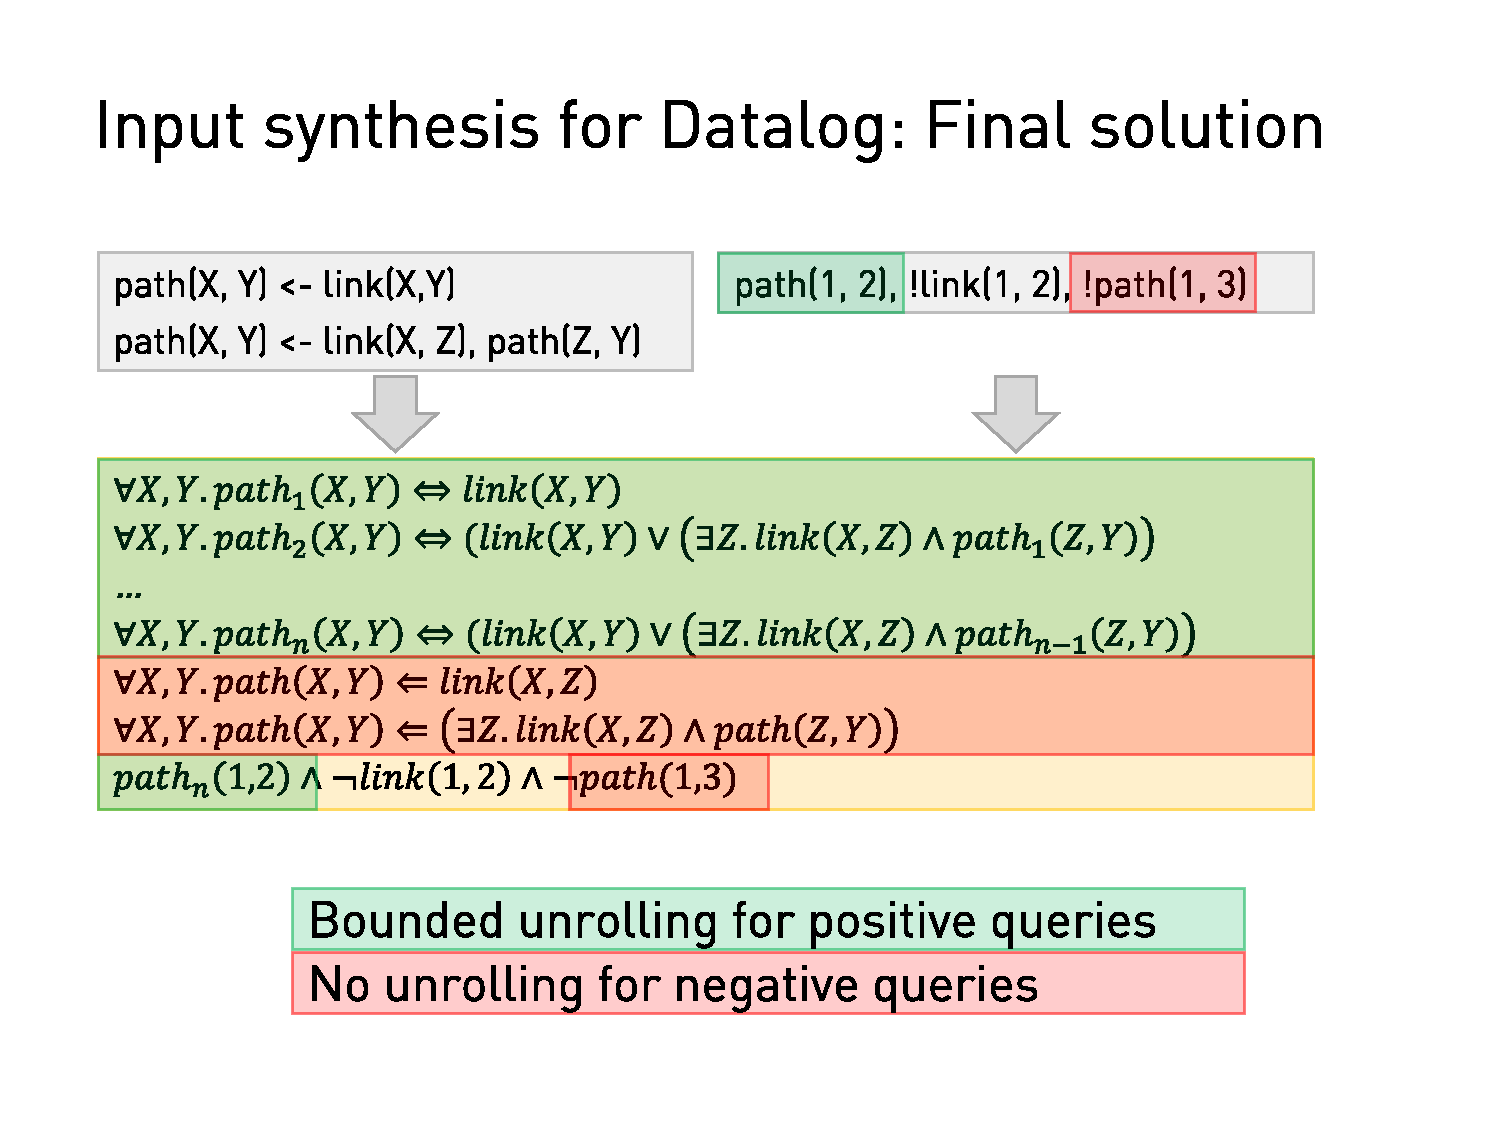
\includegraphics[width=\unitlength,page=1]{L9_InputSynthesis.pdf}}%
  \end{picture}%
\endgroup%    
\end{minipage}

\paragraph{Challenges: }Key challenge is the scaling of synthesis for OSPF protocol (takes much more computation time)

\subsection{NetComplete}
\paragraph{Sketching: } A concept to express intent
\begin{itemize}
    \item Allow users to express insight by defining the hypothesis space and bias the search.
    \item Machine helps with low-level reasoning
\end{itemize}

\paragraph{Expressing Intent}Two ways to express intent and control hypothesis space:
\begin{itemize}
    \item \textcolor{orange}{Specifications: }Define what function you actually want:
    \begin{itemize}
        \item Assertions: \texttt{assert x > y;}
        \item Concrete Examples: \texttt{x = 5 or x = 6}
        \item Function Equivalence: \texttt{blockedMatMul(Mat a, Mat b) implements matMul}
    \end{itemize}
    \item \textcolor{orange}{Holes: }To be instantiated by the synthesizer. Fragment must come from a set defined by the user. Holes define the hypothesis space.\\
    
    \begin{minipage}{\linewidth}
    \centering      
    \def\svgwidth{\linewidth}
    %% Creator: Inkscape 1.0 (4035a4fb49, 2020-05-01), www.inkscape.org
%% PDF/EPS/PS + LaTeX output extension by Johan Engelen, 2010
%% Accompanies image file 'L9_Holes.pdf' (pdf, eps, ps)
%%
%% To include the image in your LaTeX document, write
%%   \input{<filename>.pdf_tex}
%%  instead of
%%   \includegraphics{<filename>.pdf}
%% To scale the image, write
%%   \def\svgwidth{<desired width>}
%%   \input{<filename>.pdf_tex}
%%  instead of
%%   \includegraphics[width=<desired width>]{<filename>.pdf}
%%
%% Images with a different path to the parent latex file can
%% be accessed with the `import' package (which may need to be
%% installed) using
%%   \usepackage{import}
%% in the preamble, and then including the image with
%%   \import{<path to file>}{<filename>.pdf_tex}
%% Alternatively, one can specify
%%   \graphicspath{{<path to file>/}}
%% 
%% For more information, please see info/svg-inkscape on CTAN:
%%   http://tug.ctan.org/tex-archive/info/svg-inkscape
%%
\begingroup%
  \makeatletter%
  \providecommand\color[2][]{%
    \errmessage{(Inkscape) Color is used for the text in Inkscape, but the package 'color.sty' is not loaded}%
    \renewcommand\color[2][]{}%
  }%
  \providecommand\transparent[1]{%
    \errmessage{(Inkscape) Transparency is used (non-zero) for the text in Inkscape, but the package 'transparent.sty' is not loaded}%
    \renewcommand\transparent[1]{}%
  }%
  \providecommand\rotatebox[2]{#2}%
  \newcommand*\fsize{\dimexpr\f@size pt\relax}%
  \newcommand*\lineheight[1]{\fontsize{\fsize}{#1\fsize}\selectfont}%
  \ifx\svgwidth\undefined%
    \setlength{\unitlength}{720.00000454bp}%
    \ifx\svgscale\undefined%
      \relax%
    \else%
      \setlength{\unitlength}{\unitlength * \real{\svgscale}}%
    \fi%
  \else%
    \setlength{\unitlength}{\svgwidth}%
  \fi%
  \global\let\svgwidth\undefined%
  \global\let\svgscale\undefined%
  \makeatother%
  \begin{picture}(1,0.75)%
    \lineheight{1}%
    \setlength\tabcolsep{0pt}%
    \put(0,0){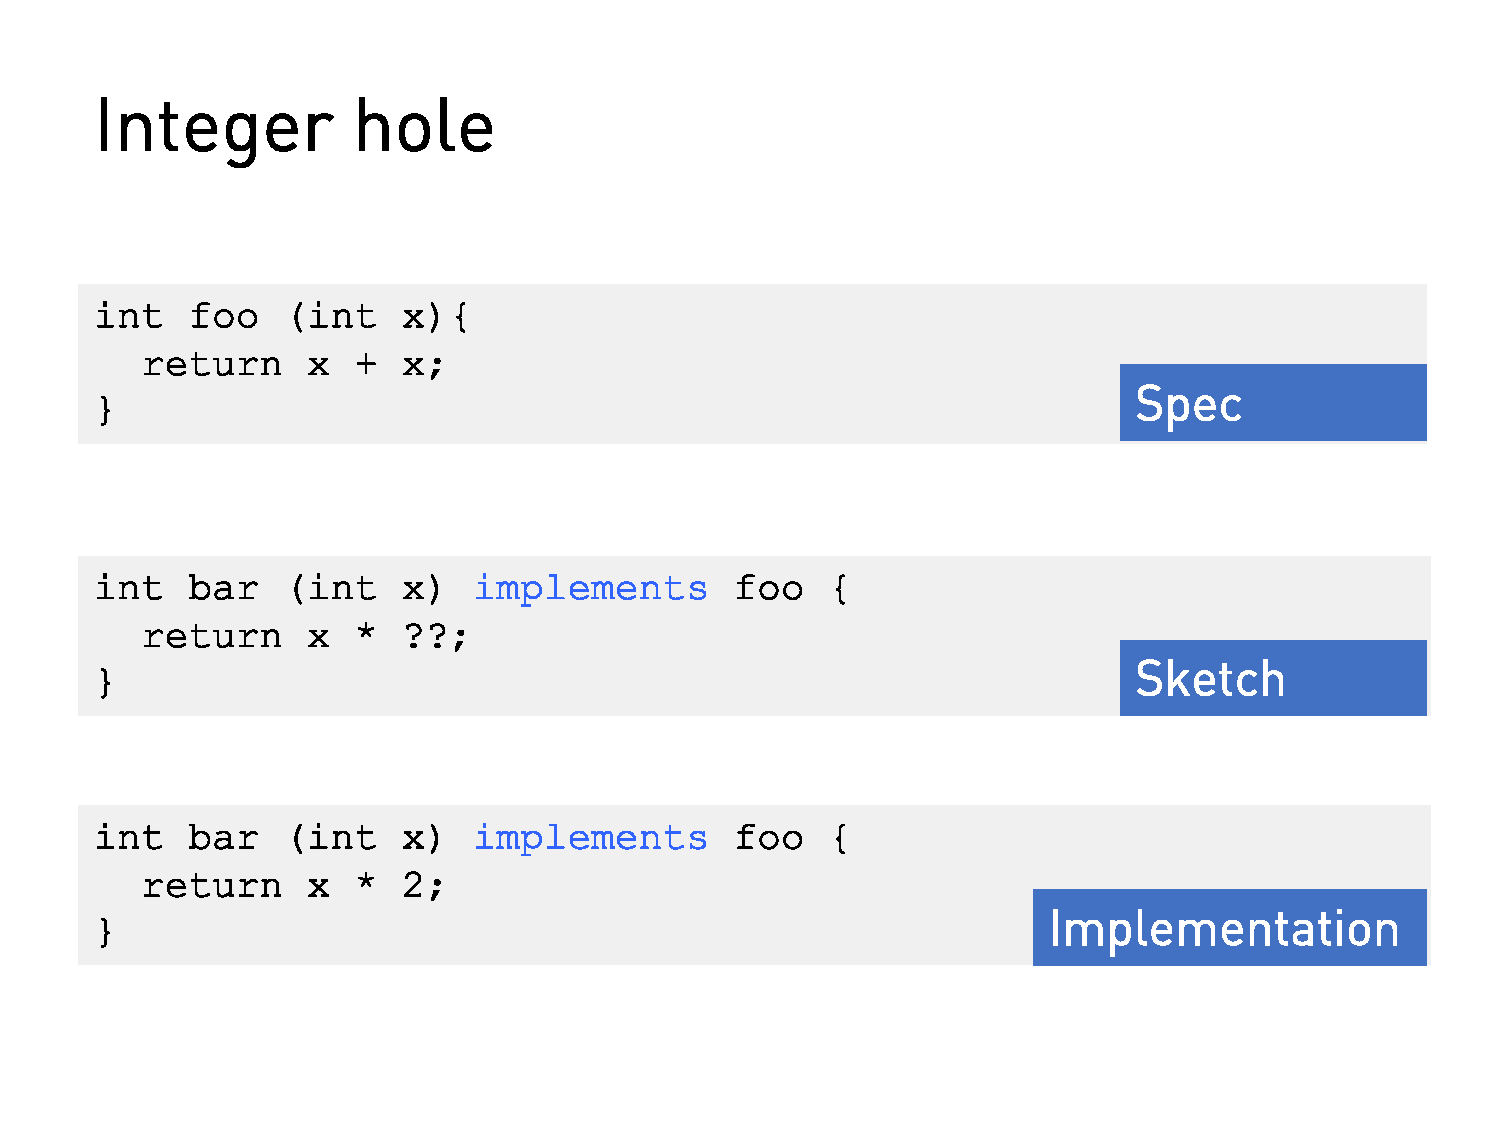
\includegraphics[width=\unitlength,page=1]{L9_Holes.pdf}}%
  \end{picture}%
\endgroup%    
    \end{minipage}

\end{itemize}

\paragraph{Synthesizing functions: } Look at slides 49ff. (chume nöd ganz drus)
\begin{enumerate}
    \item Turn holes into special inputs of the function (Control inputs C)
    \item Constraining the set of controls. Constraints are collected into a predicate Q(x,c)
    \item Synthesize function: Learning reduces to constraint satisfaction
\end{enumerate}

\paragraph{Counter-example guided inductive synthesis (CEGIS): } CEGIS aims to find the right small set of examples S so that if we learn a function F satisfying S, then F is likely to be correct on all (potentially infinite set of) examples

\begin{minipage}{\linewidth}
    \centering      
    \def\svgwidth{\linewidth}
    %% Creator: Inkscape 1.0 (4035a4fb49, 2020-05-01), www.inkscape.org
%% PDF/EPS/PS + LaTeX output extension by Johan Engelen, 2010
%% Accompanies image file 'L9_CEGIS.pdf' (pdf, eps, ps)
%%
%% To include the image in your LaTeX document, write
%%   \input{<filename>.pdf_tex}
%%  instead of
%%   \includegraphics{<filename>.pdf}
%% To scale the image, write
%%   \def\svgwidth{<desired width>}
%%   \input{<filename>.pdf_tex}
%%  instead of
%%   \includegraphics[width=<desired width>]{<filename>.pdf}
%%
%% Images with a different path to the parent latex file can
%% be accessed with the `import' package (which may need to be
%% installed) using
%%   \usepackage{import}
%% in the preamble, and then including the image with
%%   \import{<path to file>}{<filename>.pdf_tex}
%% Alternatively, one can specify
%%   \graphicspath{{<path to file>/}}
%% 
%% For more information, please see info/svg-inkscape on CTAN:
%%   http://tug.ctan.org/tex-archive/info/svg-inkscape
%%
\begingroup%
  \makeatletter%
  \providecommand\color[2][]{%
    \errmessage{(Inkscape) Color is used for the text in Inkscape, but the package 'color.sty' is not loaded}%
    \renewcommand\color[2][]{}%
  }%
  \providecommand\transparent[1]{%
    \errmessage{(Inkscape) Transparency is used (non-zero) for the text in Inkscape, but the package 'transparent.sty' is not loaded}%
    \renewcommand\transparent[1]{}%
  }%
  \providecommand\rotatebox[2]{#2}%
  \newcommand*\fsize{\dimexpr\f@size pt\relax}%
  \newcommand*\lineheight[1]{\fontsize{\fsize}{#1\fsize}\selectfont}%
  \ifx\svgwidth\undefined%
    \setlength{\unitlength}{720.00000454bp}%
    \ifx\svgscale\undefined%
      \relax%
    \else%
      \setlength{\unitlength}{\unitlength * \real{\svgscale}}%
    \fi%
  \else%
    \setlength{\unitlength}{\svgwidth}%
  \fi%
  \global\let\svgwidth\undefined%
  \global\let\svgscale\undefined%
  \makeatother%
  \begin{picture}(1,0.75)%
    \lineheight{1}%
    \setlength\tabcolsep{0pt}%
    \put(0,0){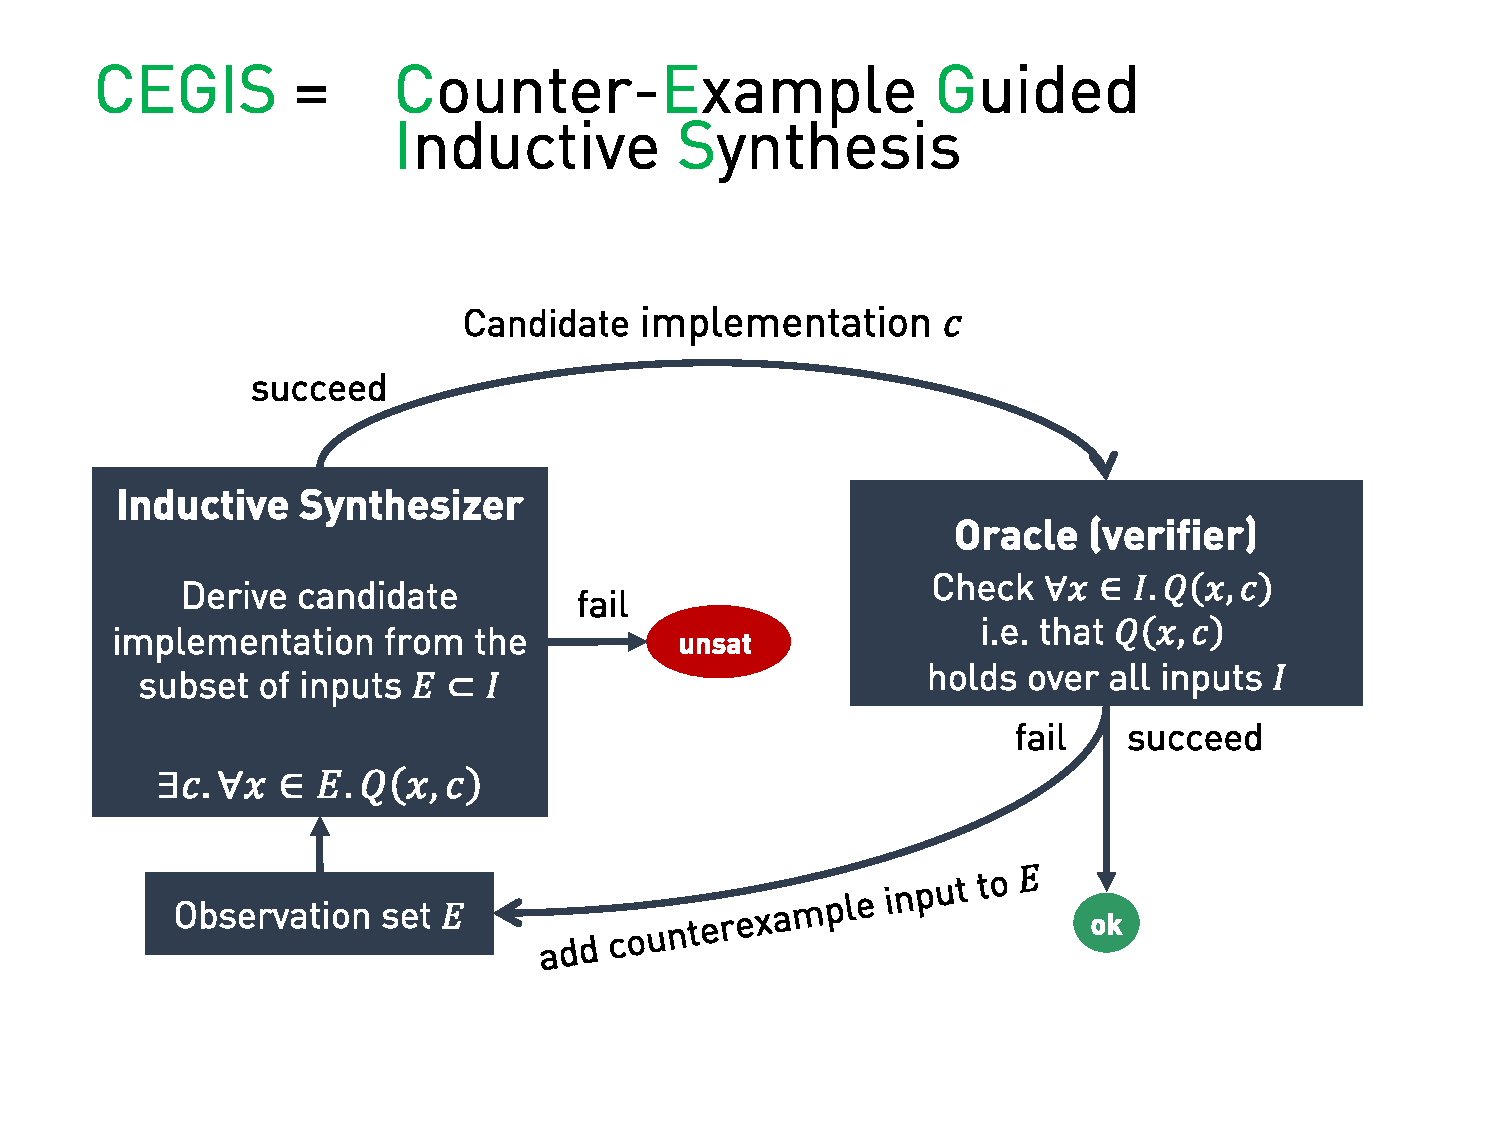
\includegraphics[width=\unitlength,page=1]{L9_CEGIS.pdf}}%
  \end{picture}%
\endgroup%
    
    \end{minipage}

\paragraph{Efficient OSPF synthesis using CEGIS: } Define logical constraints that capture the OSPF requirements. Find cost assignment f such that requirements hold. Formula given to the solver.